\documentclass[12pt]{article}
\usepackage[left=1cm, right=1cm, top=2cm,bottom=1.5cm]{geometry} 

\usepackage[parfill]{parskip}
\usepackage[utf8]{inputenc}
\usepackage[T2A]{fontenc}
\usepackage[russian]{babel}
\usepackage{enumitem}
\usepackage[normalem]{ulem}
\usepackage{amsfonts, amsmath, amsthm, amssymb, mathtools}

\usepackage{fancyhdr}
\pagestyle{fancy}
\renewcommand{\headrulewidth}{1.5pt}
\renewcommand{\footrulewidth}{1pt}

\usepackage{graphicx}
\usepackage[figurename=Рис.]{caption}
\usepackage{subcaption}
\usepackage{float}

%%Наименование папки откуда забирать изображения
\graphicspath{ {./images/} }

%%Изменение формата для ввода доказательства
\renewcommand{\proofname}{$\square$  \nopunct}
\renewcommand\qedsymbol{$\blacksquare$}

\addto\captionsrussian{%
	\renewcommand{\proofname}{$\square$ \nopunct}%
}
%% Римские цифры
\newcommand{\RN}[1]{%
	\textup{\uppercase\expandafter{\romannumeral#1}}%
}

\theoremstyle{definition}
\newtheorem{defn}{Опр:}
\newtheorem{rem}{Rm:}
\newtheorem{prop}{Утв.}	
\newtheorem{exrc}{Упр.}
\newtheorem{lemma}{Лемма}
\newtheorem{theorem}{Теорема}
\newtheorem{corollary}{Следствие}
\newtheorem{axiom}{Аксиома}
\newtheorem*{axiom*}{Аксиома}
\newenvironment{cusdefn}[1]
{\renewcommand\thedefn{#1}\defn}
{\enddefn}

\DeclareRobustCommand{\divby}{%
	\mathrel{\text{\vbox{\baselineskip.65ex\lineskiplimit0pt\hbox{.}\hbox{.}\hbox{.}}}}%
}

\newcommand{\smallerrel}[1]{\mathrel{\mathpalette\smallerrelaux{#1}}}
\newcommand{\smallerrelaux}[2]{\raisebox{.1ex}{\scalebox{.75}{$#1#2$}}}
\newcommand{\smallin}{\smallerrel{\in}}
\newcommand{\smallnotin}{\smallerrel{\notin}}


\begin{document}
	\lhead{Математический анализ - I}
	\chead{Шапошников С.В.}
	\rhead{Лекция - 8}
	
\subsection*{Пример последовательности без предела:}
	
$a_n = (-1)^n$ - нет предела.

\begin{figure}[H]
	\centering
	\includegraphics[width=0.5\textwidth]{8_1.eps}
	\caption{Последовательность $a_n = (-1)^n$}
	\label{8_1}
\end{figure}	

Докажем, что нет предела: в окрестностях $1$ и $-1$ какую бы точку не взяли $1$ или $-1$ и окрестность от нее, какой бы далекий $N$ не взяли, найдется точка, которая в этой последовательности не лежит. Для каждой точки прямой проверили, что нет предела. Но перебирать все точки последовательности и проверять это предел или нет - не очень удобное занятие.

\section*{Свойства пределов последовательностей}

\begin{theorem}\textbf{Об ограниченности}:
	Если последовательность $a_n$ - сходится (есть такое $a$, которое является пределом этой последовательности), то $a_n$ - ограничена, то есть существует отрезок, содержащий все члены последовательности.
\end{theorem}

\begin{figure}[H]
	\centering
	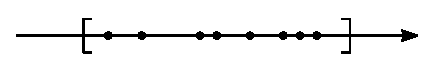
\includegraphics[width=0.34\textwidth]{8_2.eps}
	\caption{Ограниченность сходящейся последовательности}
	\label{8_2}
\end{figure}	

\begin{rem}
	В качестве такого отрезка всегда можно выбрать отрезок $[-c,c]$, где $|a_n| \leq c$.
	
	\begin{figure}[H]
		\centering
		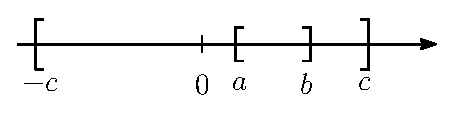
\includegraphics[width=0.34\textwidth]{8_3.eps}
		\caption{Интервал, ограничивающий последовательность}
		\label{8_4}
	\end{figure}
\end{rem}

\subsection*{Примеры}

\begin{enumerate}[label={\arabic*)}]
	\item $\dfrac{1}{n}$ - лежит в отрезке $[0,1]$ - ограниченная последовательность;
	\item $n$ - не лежит ни в каком отрезке, по аксиоме Архимеда - неограниченная последовательность;
\end{enumerate}

\begin{figure}[H]
	\centering
	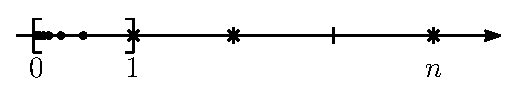
\includegraphics[width=0.4\textwidth]{8_4.eps}
	\caption{Примеры последовательностей: $\frac{1}{n}$ - ограниченная, $n$ - неограниченная}
	\label{8_3}
\end{figure}


\begin{proof}
	Пусть $a_n \to a$. Начиная с некоторого номера $n > N$ вся последовательность будет находится в интервале $(a-\varepsilon, a +\varepsilon)$ по определению. Обозначим его как $(\alpha, \beta) = (a-\varepsilon, a +\varepsilon)$. Вне этого интервала может быть только конечное число точек $a_1, a_2, \dotsc, a_N$. 
	
	\begin{figure}[H]
		\centering
		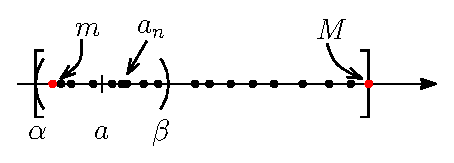
\includegraphics[width=0.34\textwidth]{8_5.eps}
		\caption{Ограниченность, сходящейся последовательности}
		\label{fig:8_5}
	\end{figure}
	
	Обозначим $m = \min\{a_1, a_2, \dotsc, a_N\}, \, M = \max\{a_1, a_2, \dotsc, a_N\}$. Возьмем следующий интервал: $$\Big[\min\{\alpha,m\}, \max\{\beta,M\}\Big]$$ - в него должны попадать все члены последовательности. Таким образом, последовательность - ограничена.
\end{proof}
	
	
\begin{theorem}\textbf{Об отделимости}: 
	Если  $\lim\limits_{n \rightarrow \infty}{a_n} = a$ и $a > 0$, то $\exists \, N\colon \, \forall n > N, \, a_n > \dfrac{a}{2} > 0$ - отделены от нуля. 
\end{theorem}

\begin{proof}
	По определению предела, $\varepsilon = \dfrac{a}{2} \Rightarrow \exists \, N \colon \forall n > N, \, |a_n - a| < \dfrac{a}{2} \Rightarrow 0 < \dfrac{a}{2} < a_n < \dfrac{3a}{2}$. 
	\begin{figure}[H]
		\centering
		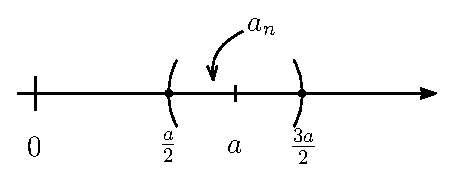
\includegraphics[width=0.34\textwidth]{8_6.eps}
		\caption{Отделимость членов последовательности}
		\label{fig:8_6}
	\end{figure}
	Таким образом, начиная с некоторого номера $N$ все элементы последовательности будут отделены от нуля.
\end{proof}
	
\begin{theorem}\textbf{Предел в неравенствах}:
	Если $\lim\limits_{n \rightarrow \infty}{a_n} = a$, $\lim\limits_{n \rightarrow \infty}{b_n} = b$ и $\exists \, N\colon \forall n > N, \, a_n \leq b_n$, то $a \leq b$
\end{theorem}

\begin{proof}
	От противного, пусть $b < a$. Тогда $\exists \, N_b \colon \forall n > N_b, \, b_n \in I_b$, $\exists \, N_a \colon \forall n > N_a, \, a_n \in I_a$.
	
	\begin{figure}[H]
		\centering
		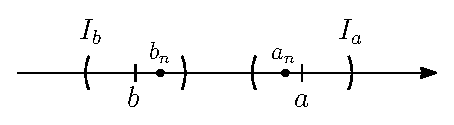
\includegraphics[width=0.34\textwidth]{8_7.eps}
		\caption{Отрезки, содержащие пределы}
		\label{fig:8_7}
	\end{figure}
	
	Пусть $n > N, N_a, N_b$, тогда по условию $a_n \leq b_n$, но по построению $I_a,\, I_b \Rightarrow a_n > b_n \Rightarrow$ противоречие. 
\end{proof}
	
\begin{rem}
	Если в условии будет $a_n < b_n$ в заключении ничего не поменяется, то есть $a \leq b$, пример $\{a_n\} = \dfrac{1}{n}, \, \{b_n\} = 0 \Rightarrow b_n < a_n$, но $b = a \Rightarrow b \leq a$.
\end{rem}
	
	
\begin{theorem}\textbf{О двух полицейских}:
	Пусть  $\lim\limits_{n \rightarrow \infty}{a_n} = a$, $\lim\limits_{n \rightarrow \infty}{b_n} = a$ и $\exists \, N \colon \forall n > N, \, a_n \leq c_n \leq b_n$, тогда $\lim\limits_{n \rightarrow \infty}{c_n} = a$.
\end{theorem}
	
\begin{proof}
$\forall (\alpha, \beta) \colon a \in (\alpha, \beta), \, \exists \, N_a \colon \forall n > N_a, \, a_n \in (\alpha,\beta), \, \exists \, N_b \colon \forall n > N_b, \, b_n \in (\alpha,\beta).$
	\begin{figure}[H]
		\centering
		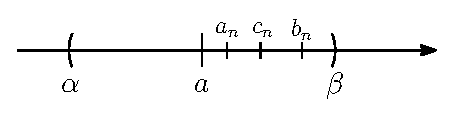
\includegraphics[width=0.34\textwidth]{8_8.eps}
		\caption{Теорема о трех милиционерах}
		\label{fig:8_8}
	\end{figure}
Возьмем $\tilde{N} = \max\{N, N_a, N_b\} \Rightarrow \forall n > \tilde{N}, \, \alpha < a_n \leq c_n \leq b_n < \beta \Rightarrow c_n \in (\alpha,\beta)$. Начиная с какого-то номера все $c_n$ лежат в интервале $(\alpha, \beta)$. А это означает  $\lim\limits_{n \rightarrow \infty}{c_n} = \lim\limits_{n \rightarrow \infty}{a_n} = \lim\limits_{n \rightarrow \infty}{b_n} = a$.
\end{proof}

\textbf{Пример}: $\lim\limits_{n \rightarrow \infty}{\sqrt[^n]{2}} = 1 ?$ Рассмотрим $2 = 1 + 1$, $\sqrt[^n]{2} > 1$, $(1+x)^n > 1+\underbrace{nx}_{y} \Rightarrow 1 + \dfrac{y}{n} \geq \sqrt[^n]{1+y} \Rightarrow$ 
$\Rightarrow 1+\dfrac{1}{n} \geq \sqrt[^n]{2} > 1$. Рассмотрим последовательности:
	
\begin{figure}[H]
	\centering
	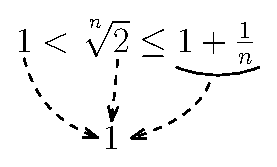
\includegraphics[width=0.2\textwidth]{8_9.eps}
	\caption{Применение теоремы о трех милиционерах}
	\label{fig:8_9}
\end{figure}
	
$a_n = 1 \rightarrow a = 1, \, b_n = 1 + \dfrac{1}{n} \rightarrow a = 1 \Rightarrow c_n = \sqrt[^n]{2} \rightarrow a = 1 $.
	
\begin{theorem}\textbf{Арифметика пределов}:
	Пусть  $\lim\limits_{n \rightarrow \infty}{a_n} = a$, $\lim\limits_{n \rightarrow \infty}{b_n} = a$. Тогда:
	\begin{enumerate}[label={\arabic*)}]
		\item  $\lim\limits_{n \rightarrow \infty}(a_n + b_n) = a + b$;
		\item $\lim\limits_{n \rightarrow \infty}(a_n \cdot b_n) = a \cdot b$;
		\item Если $b_n \neq 0$ и $b \neq 0$, то $\lim\limits_{n \rightarrow \infty}\dfrac{a_n}{b_n} = \dfrac{a}{b}$;
	\end{enumerate}
\end{theorem}

\begin{proof}
	\begin{enumerate}[label={\arabic*)}]
		\item По условию $\forall \varepsilon > 0, \exists\, N_a\colon \forall n > N_a, \, |a_n - a| < \varepsilon$, $\forall \varepsilon > 0, \exists\, N_b\colon \forall n > N_b, \, |b_n - b| < \varepsilon$
		Пусть $N = \max \{N_a, N_b\}$, тогда по неравеству треугольника:
		$$\forall n > N, \, \big|(a_n + b_n) - (a + b) \big| = \big|(a_n - a) + (b_n - b) \big|\leq |a_n - a| + |b_n - b| < 2 \varepsilon.$$
		
		Домножение константы на $\varepsilon$ не имеет значения, поскольку в определении идет $\forall \varepsilon$.
		
		\item $|a_nb_n - ab| = | a_nb_n - ab_n + ab_n -ab| \leq |b_n||a_n - a| + |a||b_n - b|$. По условию $\forall \varepsilon > 0, \exists \, N_a\colon \forall n > N_a, \, |a_n - a| < \varepsilon$, $\forall \varepsilon > 0, \exists \, N_b\colon \forall n > N_b, \, |b_n - b| < \varepsilon$. Если последовательность сходится, то она ограниченна $\Rightarrow \{b_n\}$ - ограниченная последовательность $\Rightarrow \exists\, C\colon |b_n| \leq C$. Пусть $\tilde{N} = \max \{N_a, N_b\}$, тогда 
		$$\forall n > \tilde{N}, \, |a_nb_n - ab| \leq |b_n||a_n - a| + |a||b_n - b| < C\varepsilon + |a|\varepsilon = (C + |a|)\varepsilon.$$
		
		Константа роли не играет, поэтому утверждение верно.
		
		\item Достаточно проверить, что  $\lim\limits_{n \rightarrow \infty}\dfrac{1}{b_n} = \dfrac{1}{b}$. По условию $b_n \neq 0$, пусть $b > 0$. По теореме отделимости $\exists \, N_0\colon \forall n > N_0, \, b_n > \dfrac{b}{2} > 0$. По условию $\forall \varepsilon > 0, \exists\, N_b\colon \forall n > N_b, \, |b_n - b| < \varepsilon$. 
		Пусть $\tilde{N} = \max\{N_0, N_b\}, \, \forall n > \tilde{N}, \, \bigg|\dfrac{1}{b_n} - \dfrac{1}{b} \bigg| = \dfrac{|b_n - b|}{b_n\cdot b}\underset{b_n > \frac{b}{2}}{\leq} \dfrac{|b_n - b|}{\frac{b^2}{2}}< \dfrac{2 \varepsilon}{b^2} = \dfrac{2}{b^2}\varepsilon$	
		
		Константа роли не играет, поэтому утверждение верно.
	\end{enumerate}
\end{proof}

\begin{rem}
	Почему константа не важна? По определению $\lim\limits_{n \to \infty}a_n = a \Leftrightarrow \forall \varepsilon > 0, \exists \, N \colon \forall n > N, \, |a_n -a| < \varepsilon$. Тогда если возьмем $\varepsilon = \tilde{\varepsilon}{c}$, где $c>0$, получим: $ \forall \tilde{\varepsilon} > 0, \exists \, N(\tilde{\varepsilon}c) \colon \forall n > N, \, |a_n -a| < \tilde{\varepsilon}c$.
\end{rem}

\textbf{Пример:} $\lim\limits_{n \to \infty}\dfrac{n^{2018} + n^{2017} + 1}{n^{2018} + n^{2015} + 2} = \lim\limits_{n \to \infty}\dfrac{1 + \frac{1}{n} + (\frac{1}{n})^{2018}}{1 + (\frac{1}{n})^3 + (\frac{2}{n})^{2018}} = 1$.


\subsection*{Существование пределов}

\begin{theorem}\textbf{(Вейрштрасса)}:
	Если последовательность $\{a_n\}$ не убывает и ограниченна сверху, то существует предел  $\lim\limits_{n \rightarrow \infty}{a_n}$ и этот предел равен $\sup\{a_n\}$.
	
	Если последовательность $\{a_n\}$ не возрастает и ограниченна снизу, то существует предел  $\lim\limits_{n \rightarrow \infty}{a_n}$ и этот предел равен $\inf \{a_n\}$.
\end{theorem}


\begin{figure}[H]
	\centering
	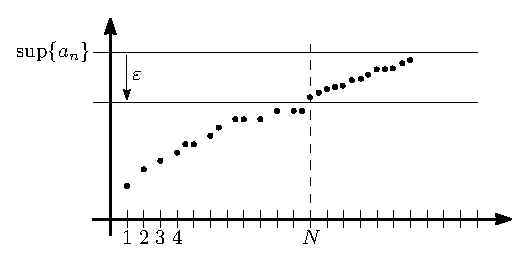
\includegraphics[width=0.45\textwidth]{8_10.eps}
	\caption{Теорема Вейрштрасса}
	\label{fig:8_12}
\end{figure}

\begin{proof}
Так как множество значенией $\{a_n\}$ ограниченно сверху, то по принципу полноты Вейрштрасса существует $\sup\{a_n\} = A$. $\forall \varepsilon > 0, \, A - \varepsilon$ - не является верхней гранью. Следовательно $\exists \, N\colon a_N > A - \varepsilon$.\\
Из-за монотонности $\{a_n\}$ видно, что $A - \varepsilon < a_N \leq a_n, \, \forall n > N$. Поэтому $\forall n > N, \, A - \varepsilon < a_n \leq A$ (так как $A$ - верхняя грань) $\Rightarrow |a_n - A| < \varepsilon$.
	
Так как множество значенией $\{a_n\}$ ограниченно снизу, то по принципу полноты Вейрштрасса существует $\inf\{a_n\} = B$. $\forall \varepsilon > 0, \, B + \varepsilon$ - не является нижней гранью. Следовательно $\exists \, N\colon a_N < B + \varepsilon$.\\
Из-за монотонности $\{a_n\}$ видно, что $a_n \leq a_N < B + \varepsilon, \, \forall n > N$. Поэтому $\forall n > N, \, B \leq a_n < B + \varepsilon$ (так как $B$ - нижняя грань) $\Rightarrow |a_n - B| < \varepsilon$.
\end{proof}

\textbf{Пример}: $a_n = \bigg(1 + \dfrac{1}{n}\bigg)^n$, проверим, что $a_n$ возрастает и ограниченна сверху.

По биному Ньютона: $$\bigg(1 + \dfrac{1}{n}\bigg)^n = \sum\limits_{k = 0}^n C_n^k \bigg(\frac{1}{n}\bigg)^k = \sum\limits_{k = 0}^n \dfrac{n\big(n-1\big)...\big(n-(k-1)\big)}{k!n^k} = \sum\limits_{k = 0}^n \dfrac{n\big(1-\frac{1}{n}\big)...\big(1-\frac{k-1}{n}\big)}{k!	}$$

так как $k$ скобочек и в каждую внесем $n$. $n$ растет $\Rightarrow 1 -\frac{m}{n}$ - увеличивается .Следовательно, каждое слагаемое растет и число слагаемых тоже растет, поэтому эта последовательность растет $\Rightarrow$\\ 
$\Rightarrow \bigg(1 + \dfrac{1}{n}\bigg)^n$ - возрастает.

Заметим, что каждое слагаемое меньше или равно $\dfrac{1}{k!} \Rightarrow \bigg(1 + \dfrac{1}{n}\bigg)^n \leq \displaystyle \sum\limits_{k = 0}^n \dfrac{1}{k!} = 1 + 1 + \dfrac{1}{2!} + \dfrac{1}{3!} + \dotsc + \dfrac{1}{n!}$.

\begin{exrc}
	$k! \geq 2^{k-1}$ - доказать по индукции.
\end{exrc}
Cледовательно 
$$1 + 1 + \dfrac{1}{2!} + \dfrac{1}{3!} + \dotsc + \dfrac{1}{n!} \leq 1  + 1 + \overbrace{\dfrac{1}{2} + \dfrac{1}{4} + \dotsc}^{\leq 1} < 3.$$
Доказали, что последовательность строго возрастает и ограниченна, a значит сходится.

\begin{defn}
	$\lim\limits_{n \rightarrow \infty}\bigg(1 + \dfrac{1}{n}\bigg)^n = e$ - число $e$. $2 < e < 3, \, e = 2.718281828\dotsc$ .
\end{defn}

\end{document}